% file: tournament_4_rep_6_2.tex
% created by Orbiter tikz interface
% creation date: Fri Nov 29 20:48:18 MST 2019
% DeviceCoordinates 0 0 1000000 1000000
% UserCoordinates 0 0 1000000 1000000
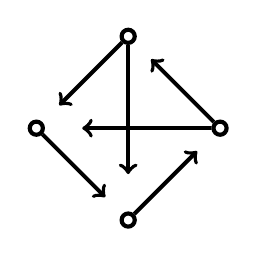
\begin{tikzpicture}[scale=0.1,line width = 1.5pt]
\draw [->,line width=0.5mm] (28.3333,16.6667) -- (19.5833,25.4167);
\draw [->,line width=0.5mm] (28.3333,16.6667) -- (10.8333,16.6667);
\draw [->,line width=0.5mm] (16.6667,5) -- (25.4167,13.75);
\draw [->,line width=0.5mm] (16.6667,28.3333) -- (7.91667,19.5833);
\draw [->,line width=0.5mm] (16.6667,28.3333) -- (16.6667,10.8333);
\draw [->,line width=0.5mm] (5,16.6667) -- (13.75,7.91667);
\filldraw[color=white] (28.3333,16.6667) circle [radius = 0.833333cm];
\draw (28.3333,16.6667) circle [radius = 0.833333cm];
\filldraw[color=white] (16.6667,28.3333) circle [radius = 0.833333cm];
\draw (16.6667,28.3333) circle [radius = 0.833333cm];
\filldraw[color=white] (5,16.6667) circle [radius = 0.833333cm];
\draw (5,16.6667) circle [radius = 0.833333cm];
\filldraw[color=white] (16.6667,5) circle [radius = 0.833333cm];
\draw (16.6667,5) circle [radius = 0.833333cm];
\end{tikzpicture}
